\chapter{Image-Based Meshing}
\label{chap:3}

\textit{Image-based meshing} is the process of generating explicitly defined volumetric meshes from imaging data for the purposes of visualization or scientific computing. The discussion will focus on generating meshes specifically from segmented image data. The term \textit{explicit} refers to defining the mesh in terms of vertex coordinates, polytopes, and the connectivity of those polytopes, as opposed to an \textit{implicit} definition in which the surface is defined as the zero-set of a 4D function. The image-based meshing process is typically separated into two major steps - 1) \textit{surface generation} and 2) \textit{CAD-based mesh generation}. Surface generation (also known as \textit{surface extraction}) is a matter of generating a watertight, manifold, polygonized surface mesh or computer-aided design (CAD) model from an image mask. CAD-based mesh generation is the task of generating a volume discretization based on the enclosing polygonized surface. Surface meshes may also be referred to as \textit{boundary representations (b-reps)}. The term \textit{b-rep} may also be used more generally though to refer to any type of surface representation, including \textit{non-uniform rational basis splines (NURBS)}, which is not typically the end goal of the surface generation step. \textit{Watertight} is the property of a surface mesh being closed - namely, if the surface were filled with water, none of it would leak out. \textit{Manifold} refers to the property of a surface being mappable to a two-dimensional plane. A non-manifold surface in practice amounts to the unintentional existence or absence of surface polytopes and/or their connectivities. It is noted that multi-material interfaces can lead to non-manifold surfaces, but the requirement that hanging nodes and self-intersecting faces are not allowed still exists in those cases.

In this chapter, image-based meshing approaches in the literature are surveyed, and a novel image-based meshing approach for binary masks is described. Specifically, a novel surface generation technique is introduced, along with its interaction with existing CAD-based meshing tools. A free image-based meshing tool that has been developed is also introduced.

%%%%%%%%%%%%%%%%%%%%%%%%%%%%%%%%%%%%%%%%%%%%%%%
%%%%%%%%%%%%%%%%%%%%%%%%%%%%%%%%%%%%%%%%%%%%%%%
\section{Image-Based Meshing Approaches}
\label{Image-Based Meshing Approaches}

A number of approaches have been pursued to tackle image-based meshing, most of which are extensions of the highly popular \textit{marching cubes} algorithm~\cite{lorensen_1987}. It assumes an implicit \textit{isosurface} exists whose volume is the union of voxels assigned the same region based on the image mask. The algorithm considers the center points of voxels in the image to be the vertices of a lattice that intersects the isosurface within each grid cell. Namely, each vertex is assigned a region number based on its associated voxel, and the edges of each cell containing the interface are bisected and used to form a triangular patch within that cell. When making use of symmetries, there are 15 predefined ways in which the isosurface can intersect a grid cell, which are stored in a look-up table. The combination of triangular patches from each grid cell form a continuous surface that is guaranteed closed and manifold~\cite{young_2008}.

The two most glaring limitations of the marching cubes algorithm are that 1) the resulting surfaces exhibit aliasing artifacts that poorly capture smooth surface and sharp features alike, and 2) the algorithm is limited to surface generation from binary masks (i.e., the algorithm cannot generate surfaces for multiple-material masks). Advances in the field of image-based meshing have mostly focused on making improvements to those two limitations - namely, generating smooth surfaces that represent the original object accurately while preserving sharp features; and generating quality surface meshes even for the case of multi-material image masks. The novel work presented in this chapter focuses on the former of the two limitations.

Updegrove \textit{et al.}~\cite{updegrove_2016} use a \textit{lofting} technique on a series of 2D segmentations to generate models of blood vessels. An approximate centerline must be drawn, and 2D segmentations are combined using spline interpolating functions to generate surfaces. Unstructured tetrahedral meshes are then generated from the surfaces. Lofting is known as a 2.5D approach, in that it cannot capture arbitrary topologies. The approach often suffers from significant loss of accuracy; the interpolating splines typically require manual selection of control points; and ambiguities can occur when stacking contours of neighboring slices~\cite{young_2008}. Most modern approaches treat an image mask as a single three-dimensional object, rather than a series of 2D masks as is done with lofting.

Young \textit{et al.}~\cite{young_2008} use a \textit{direct meshing} approach to generate meshes from multi-material image masks without the intermediate step of creating a surface mesh. The software developed by the authors - \textit{Simpleware} - is regarded among the state-of-the-art in image-based meshing tools. Young \textit{et al.} combine the surface generation and mesh generation stages into one process via their \textit{enhanced volumetric marching cubes} approach. \textit{Volumetric marching cubes} generates tetrahedral volumes based on the intersection of the isosurface with grid cells, rather than just triangular surface patches as is done in conventional marching cubes. The authors extended the volumetric algorithm to handle the intersection of up to eight regions in one grid cell - the maximum number of intersections that can occur for a Cartesian grid. The number of entries in the look-up table increases accordingly to 70. The resulting mesh is \textit{mixed hex-tet}, in that tetrahedra exist near the surface based on extended volumetric marching cubes, internal voxels are converted directly to hexahedra, and pyramidal and tetrahedral elements exist in a transitional layer in between. Additional efforts to reduce the mesh size are made by converting surface tetrahedra to hexahedra where appropriate, and by performing an octree-based approach to collect neighboring interior hexahedral elements into larger elements. Nonetheless, this \textit{grid-based} approach results in a surface mesh that is very fine, which subsequently constrains the size of interior elements in the volume mesh. Practically speaking, the resulting simulation mesh from this approach yields an intractably large number of degrees of freedom for simulation purposes. Thus, the number of points and polyhedra to define the surface must be reduced, a process known as \textit{decimation}. In turn, this allows the volumetric discretization to be coarser as well.

Indeed, the default and recommended approach in \textit{Simpleware} (known as \textit{+FE Free}) is to follow the same paradigm that has been outlined at the beginning of this chapter. Namely, the software generates a surface using extended marching cubes, performing multi-part decimation and smoothing~\cite{egst}, and finally using a conventional CAD-based tetrahedral mesher to generate fully tetrahedral meshes from the polygonized surfaces.

Meyer \textit{et al.}~\cite{meyer_2008} employ a \textit{particle-based sampling} technique for multi-material volumes. Surface samples (called \textit{particles}) are constrained to the zero-set of an implicit function, and whose distance between one another are locally adapted to create higher densities of points around surface features. A Delaunay tetrahedralization of the sampling points is computed, each tetrahedron is assigned a material label, and the surface mesh is generated by extracting the faces bounded by tetrahedra with different material labels. Finally, a conventional CAD-based tetrahedral mesher is once again employed to produce an analysis-ready mesh. The approach faithfully and robustly captures the geometries of complex material interfaces, but has debilitating performance issues, even by the own admission of the authors.

A number of other techniques have been published on the topic of image-based meshing, often times coming from completely different perspectives on the problem~\cite{bronson_2014,fang_2009,boissonnat_2009,zhao_2016}. Although several of the works presented here and otherwise attempt to generate surfaces for multi-material image masks, a great deal of effort and applicability still exists for generating high quality surfaces (and resulting meshes) from binary image masks. This will be the focus of the remainder of this chapter.

%%%%%%%%%%%%%%%%%%%%%%%%%%%%%%%%%%%%%%%%%%%%%%%
%%%%%%%%%%%%%%%%%%%%%%%%%%%%%%%%%%%%%%%%%%%%%%%
\section{Surface Generation}
\label{Surface Generation}

The most straightforward appraoch to surface generation of binary image masks simply applying the marching cubes algorithm. As alluded to in the previous section, though, surfaces generated by the marching cubes algorithm still very much have a ``Lego-like'' appearance to them, making them grossly inadequate for any simulation problem, especially one involving contact. Thus, the surface must be smoothed, hopefully using a technique that attempts to preserve the volume of the original object such as \textit{HC Laplacian smoothing}~\cite{vollmer_1999} or \textit{Taubin smoothing}~\cite{taubin_1995}. Nonetheless, the step-like appearance of surfaces extracted by marching cubes often requires a degree of smoothing that causes a significant loss in features of the desired surface, and/or the surface to become non-manifold. Sophisticated surface generation techniques attempt to generate a surface that preserves both the smooth and sharp features of the original object surface.

Labsik \textit{et al.}~\cite{labsik_2002} extract a coarse resolution surface using marching cubes, followed by iteratively remeshing to finer resolutions where features exist. Kobbelt \textit{et al.}~\cite{kobbelt_2001} retain sharp features from binary image masks by modifying the marching cubes algorithm in two ways: by enhancing the discrete distance field that defines the underlying isosurface of the image mask, and by adding additional sample points to detect edges and corners. Depending on the application, though, surface smoothness can often be a higher priority when extracting the surface. Lempitsky~\cite{lempitsky_2010}, for example, modify the isosurface function and solve a convex quadratic optimization problem for each grid cell to enforce higher-order smoothness.

The approach outlined herein involves generating a high-quality point cloud that approximates the interface, followed by a  \textit{surface reconstruction} technique based on Voronoi partitioning, where surface reconstruction is the process of generating watertight, explicit, manifold surfaces from \textit{point cloud} data. The approach attempts to create smooth surfaces without oversmoothing, and has the hooks in place to capture sharp features as well.

%%%%%%%%%%%%%%%%%%%%%%%%%%%%%%%%%%%%%%%%%%%%%%%
%%%%%%%%%%%%%%%%%%%%%%%%%%%%%%%%%%%%%%%%%%%%%%%
\subsection{Point Cloud Generation}
\label{Point Cloud Generation}

Given a segmented image, we seek to generate an \textit{oriented point cloud} to approximate the surface of the object of interest. A point cloud is oriented if the surface normal data is included at each point in addition to spatial coordinates. To compute the point cloud, the image mask is sampled with overlapping \textit{windows} to locally approximate material interfaces. For each three-dimensional window, the following tasks are performed:
\begin{itemize}[noitemsep]
  \item Determine whether the window involves an interface
  \item Approximate the interface via functional minimization
  \item Place interface a point and associated normal based on the interface
\end{itemize}
The basic sequence is shown in 2D in panels (a-c) of~\figref{vor}. Each step will be described in turn.

\begin{figure}[ht]
\centering
\subfigure[]{%
		
\includegraphics[scale=0.57]{media/2-shabaka/1-vor/dem1.png}
\label{fig:vor1}}
\subfigure[]{%
		\includegraphics[scale=0.57]{media/2-shabaka/1-vor/dem2.png}
\label{fig:vor2}}
\subfigure[]{%
		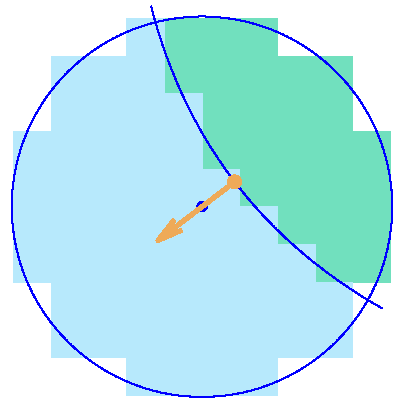
\includegraphics[scale=0.57]{media/2-shabaka/1-vor/dem3.png}
\label{fig:vor3}}
\subfigure[]{%
		\includegraphics[scale=0.57]{media/2-shabaka/1-vor/dem4.png}
\label{fig:vor4}}
%
\caption{(a) Sample window of segmented image, (b) interface approximation, (c) point/normal placement, and d) Voronoi site placement. Green voxels belong to the material of interest \textit{m} and blue voxels are void. }
\label{fig:vor}
\end{figure}

\subsubsection{Window Selection}

Define the set of all voxels in a segmented image as $\mathcal{I}$. The segmented image  $\mathcal{I}$ is sampled with overlapping windows, each of which is a voxelized sphere with voxel radius $R_{\mathcal{W}}$. The sampling distance between adjacent windows is $d_{\mathcal{W}}$. The set of voxels in a particular window is defined as $\mathcal{W}$, and the number of voxels in that window is $W$. Define the set of voxels in $\mathcal{W}$ that belong to material $m$ to be $\mathcal{M}$, and the number of voxels in $\mathcal{M}$ to be $M$. A window $\mathcal{W}$ is deemed acceptable if it satisfies certain threshold requirements. Define $k_{\mathcal{M}}$ as the ratio of voxels in $\mathcal{M}$ to the voxels in $\mathcal{W}$, i.e., the ratio $ M/W$. For a threshold value $\overline{k}_{\mathcal{M}}$, the window is discarded if $k_{\mathcal{M}} > \overline{k}_{\mathcal{M}}$ or $k_{\mathcal{M}} < 1 - \overline{k}_{\mathcal{M}}$. Thus, further calculations are only performed if there are enough voxels of material \textit{m} and of void to justify approximating a material interface. Refer to~\tabref{window} for a list of these variables and their descriptions. 

\begin{table}[htbp!]
 \centering
   \begin{tabular}{|c||c|}
   \hline
   {\textbf{Variable}} & \textbf{Description} \\ \hline \hline
   $\mathcal{I}$ & set of all voxels in a segmented image \\ \hline
   $\mathcal{W}$ & set of all voxels in a window \\ \hline
   $m$ & material of interest \\ \hline
   {$k_{\mathcal{M}}$} & ratio of voxels in $\mathcal{M}$ to voxels in $\mathcal{W}$\\ \hline
   {$\overline{k}_{\mathcal{M}}$ \rule{0mm}{4mm}} & threshold value for $k_{\mathcal{M}}$ \\ \hline 
   $R_{\mathcal{W}}$ & window radius (in voxels) \\ \hline
   $d_{\mathcal{W}}$ & sampling distance between adjacent windows (in voxels) \\ \hline  
\end{tabular}
\caption{List of variables for window selection}
\label{tab:window}
\end{table}

\subsubsection{Interface Approximation}

For a particular window $\mathcal{W}$, we seek to approximate the interface between voxels belonging to $\mathcal{M}$ and voxels belonging to $\mathcal{W} \setminus \mathcal{M}$ by a surface $\mathcal{S}$. Assuming $\mathcal{W}$ has been deemed acceptable, an approximating sphere $\mathcal{D}$ of radius $R$ is defined, such that the center and volume of this sphere match the center and volume of the window $\mathcal{W}$.

Define $\Omega_p$ as the physical space covered by the voxels belonging to $\mathcal{M}$. Define $\Omega$ as the physical space covered by an approximating lens to $\Omega_p$, determined by the space enlosed by $\mathcal{D}$ and $\mathcal{S}$. The surface $\mathcal{S}$ is determined by minimizing the error in certain geometric properties between $\Omega$ and $\Omega_p$~(see~\figref{figure3}).

\begin{figure}[ht]
\centering
\subfigure[Window $\mathcal{W}$]{%
		\includegraphics[scale=0.72]{media/om/dem2.pdf}
\label{fig:subfigure2}}
\subfigure[Approximating sphere $\mathcal{D}$]{%
		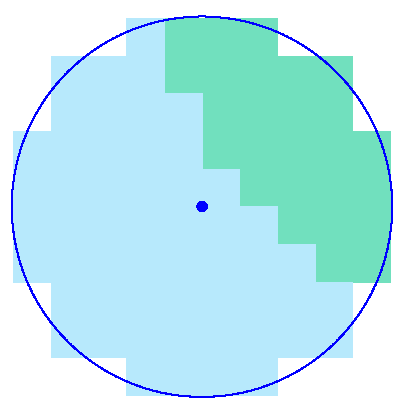
\includegraphics[scale=0.72]{media/om/dem3.pdf}
\label{fig:subfigure3}}

\subfigure[Approximating surface $\mathcal{S}$]{%
		\includegraphics[scale=0.72]{media/om/dem4.pdf}
\label{fig:subfigure4}}
\subfigure[voxelated region $\Omega_p$]{%
		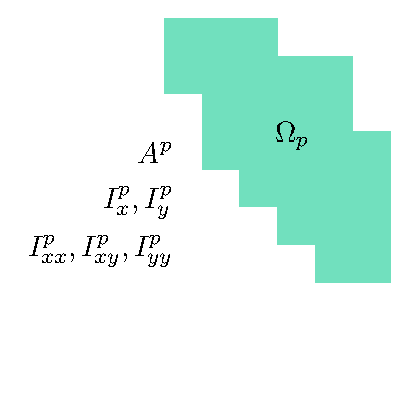
\includegraphics[scale=0.72]{media/om/omp.pdf}
\label{fig:subfigure5}}
\subfigure[Approximating lens $\Omega$]{%
		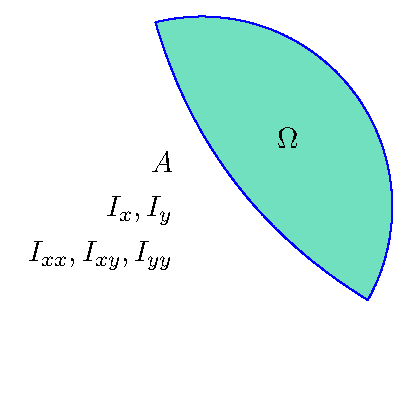
\includegraphics[scale=0.72]{media/om/om.pdf}
\label{fig:subfigure6}}

\caption{Interface approximation demonstrated in 2D}
\label{fig:figure3}
\end{figure}

The open surface $\mathcal{S}$ that approximates the interface takes an assumed form - for these purposes the interface is assumed to be a plane. If the center of the window is defined to be the origin, the interface takes the form $x' = d$, where $(x',y',z')$ are in a rotated coordinate system and $d$ is the perpendicular distance from the plane to the origin~(see~\figref{quad}).

\begin{figure}[ht!]
	\centering
		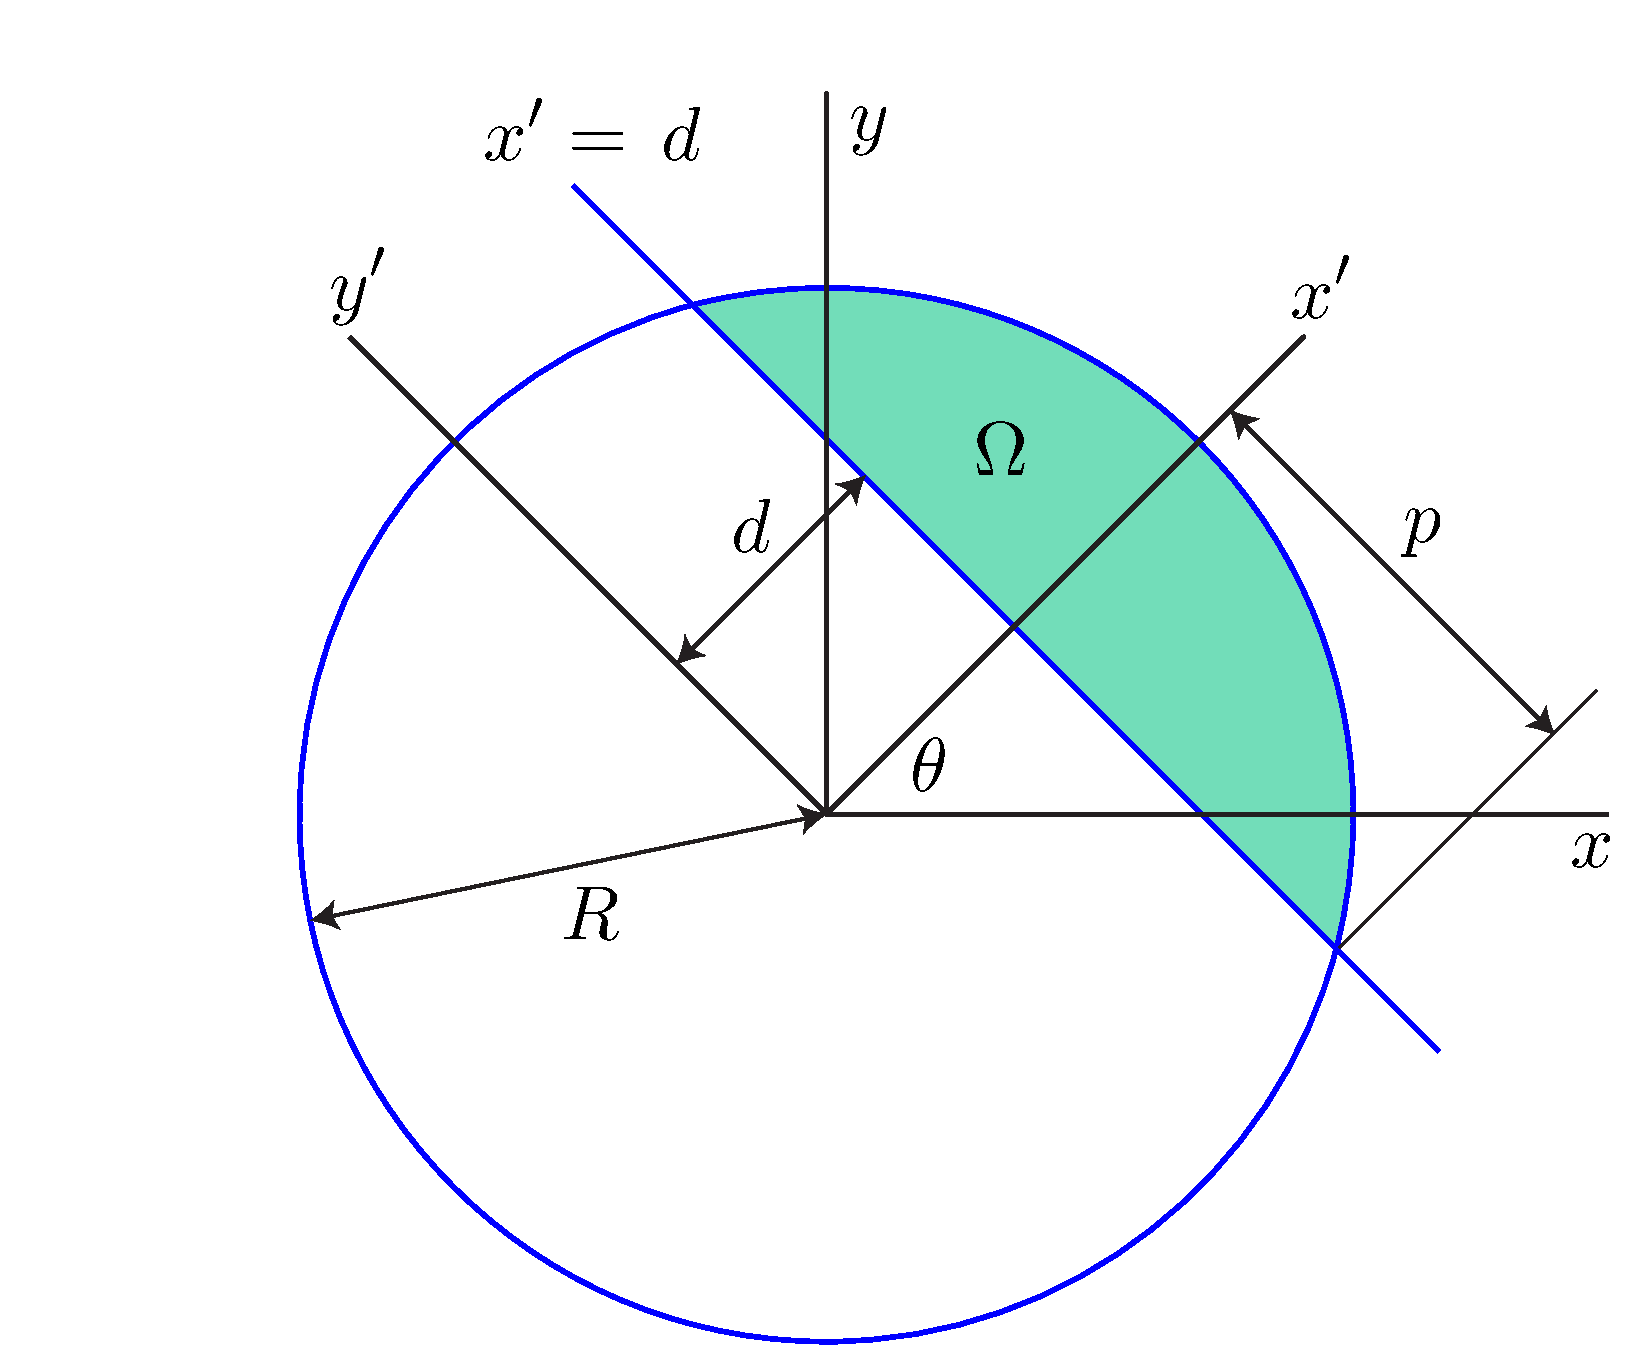
\includegraphics[scale=0.3]{media/om/window.pdf}
	\caption{Plane interface approximation demonstrated in 2D}
	\label{fig:quad}
\end{figure}

Define the following moments of volume for $\Omega_p$:
\begin{alignat}{5}
&{} &&V^p = \int_{\Omega_p}dv &&{} \\
I_{x\phantom{z}}^p &= \int_{\Omega_p}xdv, &&I_{y\phantom{z}}^p = \int_{\Omega_p}ydv, &&I_{z\phantom{z}}^p = \int_{\Omega_p}zdv \\
I^p_{xy} &= \int_{\Omega_p}xydv, &&I^p_{xz} = \int_{\Omega_p}xzdv, &&I^p_{yz} = \int_{\Omega_p}yzdv \\
I^p_{xx} &= \int_{\Omega_p}(y^2 + z^2)dv, \text{\ \ \ \ \ \ }&&I^p_{yy} = \int_{\Omega_p}(x^2 + z^2)dv, \text{\ \ \ \ \ \ }&&I^p_{zz} = \int_{\Omega_p}(x^2 + y^2)dv
\end{alignat}
And similarly for $\Omega$:
\begin{alignat}{5}
&{} &&V = \int_{\Omega}dv &&{} \\
I_{x\phantom{z}} &= \int_{\Omega}xdv, &&I_{y\phantom{z}} = \int_{\Omega}ydv, &&I_{z\phantom{z}} = \int_{\Omega}zdv \\
I_{xy} &= \int_{\Omega}xydv, &&I_{xz} = \int_{\Omega}xzdv, &&I_{yz} = \int_{\Omega}yzdv \\
I_{xx} &= \int_{\Omega}(y^2 + z^2)dv, \text{\ \ \ \ \ \ }&&I_{yy} = \int_{\Omega}(x^2 + z^2)dv, \text{\ \ \ \ \ \ }&&I_{zz} = \int_{\Omega}(x^2 + y^2)dv
\end{alignat}
For the purposes of computing the error functional, define the following quantities:
\begin{alignat}{3}
f^p &= V^p, \text{\ \ \ \ \ }&&f(d,\psi,\theta) = V \\
\bm{g}^p &= \left[\begin{array} {ccc} {I_x^p} \\ {I_y^p} \\ {I_z^p} \end{array} \right], \text{\ \ \ \ \ }&&\bm{g}(d,\psi,\theta) = \left[\begin{array} {ccc} {I_x} \\ {I_y} \\ {I_z} \end{array} \right] \\
\bm{h}^p &= \left[\begin{array} {ccc} {I_{xx}^p} & {-I_{xy}^p} & {-I_{xz}^p}\\ {-I_{xy}^p} & {I_{yy}^p} & {-I_{yz}^p} \\ -{I_{xz}^p} & {-I_{yz}^p} & {I_{zz}^p} \end{array} \right],\text{\ \ \ \ \ \ \ }&&\bm{h}(d,\psi,\theta) = \left[\begin{array} {ccc} {I_{xx}} & {-I_{xy}} & {-I_{xz}}\\ {-I_{xy}} & {I_{yy}} & {-I_{yz}} \\ -{I_{xz}} & {-I_{yz}} & {I_{zz}} \end{array} \right]
\end{alignat}
Define the relative errors as:
\begin{align}
e_0(d,\psi,\theta) &=  \sqrt{\frac{(f - f^p)^2}{(f^p)^2}} \\
e_1(d,\psi,\theta) &=  \sqrt{\frac{(g_i - g_i^p)(g_i - g_i^p)}{g_i^{p}g_i^{p}}} \\
e_2(d,\psi,\theta) &=  \sqrt{\frac{(h_{ij} - h_{ij}^p)(h_{ij} - h_{ij}^p)}{h_{ij}^{p}h_{ij}^{p}}}
\end{align}
Finally, we define the relative error functional as follows:
\begin{align}
\mathcal{F}(d,\psi,\theta) = \beta_0e_0 + \beta_1e_1 + \beta_2e_2
\end{align}
where $e_0$, $e_1$, and $e_2$ are relative errors between the zeroth, first, and second order moments of volume of $\Omega_p$ and $\Omega$, respectively. They are functions of the interface parameters $d$, $\psi$, and $\theta$, where $\psi$ and $\theta$ are the yaw and pitch angles defining the plane. The values $\beta_0$, $\beta_1$, and $\beta_2$ are weighting coefficients, where $\beta_2 = 1 - \beta_0 - \beta_1$, and $\beta_i \in [0, 1]$. We seek the solution to the following unconstrained minimization problem: $\displaystyle \min_{d, \psi, \theta} \mathcal{F}(d,\psi,\theta)$, which can be solved by a variety of well-established techniques.

The subplex search method~\cite{rowan} is used to determine the functional minimum using an implementation in the package \textit{NLopt}~\cite{nlo}. The method is a \textit{derivative-free} method that is well suited for optimizing objective functions that are noisy or discontinuous. It was selected as the optimization approach due to the existence of square roots in the objective function, and the fact that robustness to a variety of inputs was the highest priority in developing the algorithm. The performance of the point generation algorithm was not sacrificed as a result of the choice. A convergence tolerance $\varepsilon$ is defined such that on successive iterations, $\left| \mathcal{F}_{i+1} - \mathcal{F}_{i}\right| < \epsilon$, where the subscript corresponds to the iteration number. Additionally, the solution is only accepted if the error functional is below a specified value $\overline{\mathcal{F}}$, that is, $\Omega$ approximates $\Omega_p$ to a satisfactory degree. Specifically, we require that once convergence has been satisfied, the criterion $\mathcal{F} < \overline{\mathcal{F}}$ must also be met for the point and normal to be retained. In this way, outliers in which the error minimization performs poorly are discarded. This typically occurs in regions of high curvature, as a plane approximates such an interface poorly. The point cloud is dense enough that simply discarding these points is not cause for concern.

The geometric quantities of $\Omega_p$ are computed based on a straightforward use of voxel dimensions and the parallel axis theorem. The geometric quantities of $\Omega$, on the other hand, are computed based on an intricate dependence on $d$, $\psi$, and $\theta$. The moments of volume are first computed in the rotated coordinate frame:

\begin{align}
p &= \sqrt{R^2 - d^2} \\
V^* &= 2\pi\left[-\frac{1}{2}dp^2 + \frac{1}{3}R^3 - \frac{1}{3}(R^2 - p^2)^{3/2} \right] \\
I^*_{x'x'} &= \frac{\pi}{30}\left[-15dp^4 + \sqrt{R^2-p^2}\left(12p^4 - 4p^2R^2 - 8R^4\right) + 8R^5 \right] \\
\begin{split}
I^*_{y'y'} &= \frac{\pi}{480}\Big[-160d^3p^2 + 128R^5 - \sqrt{R^2-p^2}\left(128R^4 - 96p^2R^2 - 32p^4\right) - 120dp^4 \Big]
\end{split}
\end{align}
\begin{align}
V &=  \begin{cases}
      V^*, & \text{if}\ d \geq 0 \\
      V^* + \frac{4\pi}{3}\left(R^2-p^2\right)^{3/2}, & \text{otherwise}
    \end{cases} \\
I_{x'} &= \frac{\pi}{4}\left[2p^2(R^2-d^2) - p^4 \right]\\
I_{y'} &= I_{z'} = 0 \\
I_{x'y'} &= I_{x'z'} = I_{y'z'} = 0 \\
I_{x'x'} &=  \begin{cases}
      I^*_{x'x'}, & \text{if}\ d \geq 0 \\
       I^*_{x'x'} + \frac{4\pi}{15}(R^2-p^2)^{3/2}(3p^2+2R^2), & \text{otherwise}
    \end{cases} \\
I_{y'y'} &=  \begin{cases}
     I^*_{y'y'}, & \text{if}\ d \geq 0 \\
     I^*_{y'y'} + \frac{2\pi}{15}(R^2-p^2)^{3/2}(p^2+4R^2), & \text{otherwise}
    \end{cases} \\
I_{z'z'} &= I_{y'y'}
\end{align}

Note (unsurprisingly) certain moments of volume exhibit symmetries in regard to the $y'$ and $z'$ axes. Note also that additional terms may exist if $d$ is negative. Finally, the moments of volume are rotated from the prime coordinate frame to the original desired coordinate frame where moments of volume of $\Omega_p$ were computed. Note the rotation is not the same for zeroth, first, and second moments.

\begin{align}
\bm{R} &= \left[\begin{array} {ccc} {\cos\psi\cos\theta} & {-\sin\psi} & {\cos\psi\sin\theta}\\ {\sin\psi\cos\theta} & {\cos\psi} & {\sin\psi\sin\theta} \\
{-\sin\theta} & {0} & {\cos\theta}\end{array} \right] \\
\left[\begin{array} {ccc} {I_x} \\ {I_y} \\ {I_z} \end{array} \right] &= \bm{R} \left[\begin{array} {ccc} {I_{x'}} \\ {I_{y'}} \\ {I_{z'}} \end{array} \right]\\
\bm{I}' &= \left[\begin{array} {ccc} {I_{x'x'}} & {-I_{x'y'}} & {-I_{x'z'}}\\ {-I_{x'y'}} & {I_{y'y'}} & {-I_{y'z'}} \\ -{I_{x'z'}} & {-I_{y'z'}} & {I_{z'z'}} \end{array} \right] \\
\bm{I} &= \bm{R}\bm{I}'\mathbf{R}^T = \left[\begin{array} {ccc} {I_{xx}} & {-I_{xy}} & {-I_{xz}}\\ {-I_{xy}} & {I_{yy}} & {-I_{yz}} \\ -{I_{xz}} & {-I_{yz}} & {I_{zz}} \end{array} \right]
\end{align}

The solution to the minimization problem yields the values $d$, $\psi$, and $\theta$ that determine the optimally oriented surface $\mathcal{S}$, from which the interface point and normal are defined. Refer to~\tabref{surface} for a summary of variables used in approximating the interface.

\begin{table}[htbp!]
 \centering
   \begin{tabular}{|c||c|}
   \hline
   {\textbf{Variable}} & {\textbf{Description}} \\ \hline \hline
   $\mathcal{D}$ & approximating sphere to $\mathcal{W}$ \\ \hline
   $\mathcal{S}$ & surface approximating interface of interest \\ \hline      
   $R$ & radius of $\mathcal{D}$ \\ \hline   
   $\Omega_p$ & physical space covered by voxels belonging to $\mathcal{W}$ \\ \hline
   $\Omega$ & physical space covered by approximating lens of $\Omega_p$ \\ \hline      
   $(x,y,z)$ & axes aligned with image scan, whose origin is at the center of $\mathcal{W}$\\ \hline
   \multirow{2}{*}{$(x',y',z')$} & orthogonal axes whose origin is at the center of window $\mathcal{W}$,\\
   {} & where $x'$ passes through the centroid of $\Omega$ \\ \hline   
   $d$ & perpendicular distance from center of $\mathcal{D}$ to plane $\mathcal{S}$  \\ \hline
   $\psi$ & yaw angle of rotation between $(x,y,z)$ and $(x',y',z')$ axes \\ \hline   
   $\theta$ & pitch angle of rotation between $(x,y,z)$ and $(x',y',z')$ axes \\ \hline
   $V^p$ & volume of $\Omega_p$ \\ \hline
   $I_{x}^p, I_y^p$ & first moments of volume of $\Omega_p$ \\ \hline     
   $I_{xy}^p, I_{xz}^p, I_{yz}^p$ & products of volume of $\Omega_p$ \\ \hline      
   $I_{xx}^p, I_{xy}^p, I_{yy}^p$ & second moments of volume of $\Omega_p$ \\ \hline
   $V$ & volume of $\Omega$ \\ \hline
   $I_{x}, I_y$ & first moments of volume of $\Omega$ \\ \hline
   $I_{xy}, I_{xz}, I_{yz}$ & products of volume of $\Omega$ \\ \hline   
   $I_{xx}, I_{xy}, I_{yy}$ & second moments of volume of $\Omega$ \\ \hline
   $e_0$ & relative error in zeroth moment of volume \\ \hline
   $e_1$ & relative error in first moment of volume \\ \hline
   $e_2$ & relative error in second moment of volume \\ \hline   
   $\beta_0$ & functional weighting coefficient for zeroth moment of volume error \\ \hline
   $\beta_1$ & functional weighting coefficient for first moment of volume error \\ \hline
   $\beta_2$ & functional weighting coefficient for second moment of volume error \\ \hline 
   $\varepsilon$ & tolerance for minimization of functional $\mathcal{F}$ \\ \hline
   $\overline{\mathcal{F}}$ \rule{0mm}{4mm} & largest acceptable value of functional $\mathcal{F}$ \\ \hline        
\end{tabular}
\caption{List of variables for interface approximation}
\label{tab:surface}
\end{table}

\subsubsection{Interface Point and Normal Placement}

Once the parameters $d$, $\psi$, and $\theta$ are selected to fully define the surface that approximates the interface, a point location and outward normal are determined. The outward pointing normal is defined from the transformation of the $x$ axis to the $x'$ axis, i.e., the first column of matrix $\bm{R}$: $\bm{n} = -(\cos\psi\cos\theta,\text{\ }\sin\psi\cos\theta,\text{\ }-\sin\theta)$. With the origin at the center of sphere $\mathcal{D}$, the location of the interface normal is then simply $\mathbf{x}_p = -d\bm{n}$.

%%%%%%%%%%%%%%%%%%%%%%%%%%%%%%%%%%%%%%%%%%%%%%%
%%%%%%%%%%%%%%%%%%%%%%%%%%%%%%%%%%%%%%%%%%%%%%%
\subsection{Surface Reconstruction}
\label{Surface Reconstruction}

Surface reconstruction is the process of generating closed, manifold, polygonized surfaces from point clouds. The literature typically expects a dense, noisy population of points that come from laser-based scanners. The proposed algorithm does not in general produce a point cloud as dense as do laser scanners, but a brief review of surface reconstruction techniques is still informative.

Among the most well known surface reconstruction algorithms are the \textit{Power Crust} and \textit{Poisson surface reconstruction} techniques. Amenta \textit{et al.}~\cite{amenta_2001} present the \textit{Power Crust} algorithm for reconstructing watertight surfaces from unoriented point clouds. It approximates the medial axis transform from the point cloud, followed by an inverse transform to produce a piecewise-linear surface approximation. The algorithm does not perform well when the point set is not sufficiently dense, and performed quite poorly for point clouds generated from the algorithm described in the previous section. Kazhdan \textit{et al.} present \textit{Poisson surface reconstruction}~\cite{kazhdan_2008} and subsequently \textit{screened Poisson surface reconstruction}~\cite{kazhdan_2013} for oriented point clouds. They compute an indicator function defined as 1 at points inside the surface and 0 for points outside, whose gradient best approximates the vector field defined by the oriented point cloud. This amounts to solving a Poisson problem for an implicit indicator function, followed by application of marching cubes to polygonize the surface. The \textit{screened} approach provides a soft constraint that encourages the reconstructed isosurface to pass through the input points. In practice, the screened approach is significantly more robust than the original approach in terms of generating manifold surfaces from complex point clouds. The technique produces smooth surfaces that exhibit a resiliency to noise, outliers, and lack of data that is superior to any other technique experimented with.

Many other surface reconstruction approaches exist, including those making use of moving least squares, Delaunay and Voronoi constructions, and variational approaches~\cite{berger}. A novel approach that utilizes \textit{Voronoi partitioning}, and that is tuned for the type of noise and point density coming from the point cloud generation algorithm in the previous section, is presented as an alternative to these approaches.

The proposed surface reconstruction technique relies on constructing a Voronoi diagram, which for our purposes is a nearest neighbor partitioning of $\mathbb{R}^3$ based on a set of input \textit{Voronoi sites}. The desired output from a Voronoi partition is a mesh, namely a set of points, edges, facets, and cells that discretize space. Define a half plane $D(\bm{p},\bm{q})$ comprising all points $\bm{x}$ closer to site $\bm{p}$ than site $\bm{q}$:
\begin{equation}
D(\bm{p},\bm{q}) = \{\bm{x} \mid d(\bm{p},\bm{x}) \leq d(\bm{q},\bm{x})\}
\end{equation}
where a distance function $d$ must be defined. Although there are instances of more exotic distance functions, the Euclidean distance will be used for these purposes. The \textit{Voronoi cell} $V(\bm{p})$ associated with site $\bm{p}$ is the set of points inside the intersection of all half planes involving site $\bm{p}$ and all other sites in the set of sites $\mathcal{P}$:
\begin{equation}
V(\bm{p}) = \bigcap \limits_{\bm{q} \in \mathcal{P}, \bm{q} \neq \bm{p}} D(\bm{p},\bm{q})
\end{equation}
A number of important properties exist for Voronoi partitions and its dual \textit{Delaunay tesselation}, but the one of most importance for these purposes is that the extracted surface of a set of Voronoi cells connected by shared facets is watertight and manifold. Several important considerations must be made in constructing a Voronoi partition, including handling degenerate and near-degenerate cases, the data schema and order of construction of the connected polytopes that comprise the partition, and the
performance of the algorithm. Refer to Aurenhammer~\cite{aurenhammer_1991} for a detailed survey of the mathematical and algorithmic approaches to Voronoi diagrams.

The proposed technique involves the following steps, to be described in turn:
\begin{itemize}[noitemsep]
\item Generate Voronoi site set from oriented point cloud and perform Voronoi partition of image
\item Define b-rep as the set of facets that share Voronoi sites with different material type, and perform cleanup on that surface
\item Decimate, or coarsen, the surface to a more tractable mesh resolution
\end{itemize}

\subsubsection{Voronoi Site Generation and Voronoi Partitioning}

Given the location of an interface point $\bm{x}_p$ and orientation of its corresponding normal $\bm{n}$, a pair of Voronoi sites are placed on either side of the point along the line of action of the normal (see ~\figref{vor4}). They are separated from the point by a distance $b$. Thus, their locations are $\bm{x}_p \pm b \bm{n}$. The two Voronoi sites are assigned material types. For the two-material case that is considered here, the site corresponding to the position $\bm{x}_p - b\bm{n}$ is \textit{inside} $\Omega$, and thus is assigned material $m$. The site corresponding to the position $\bm{x}_p + b\bm{n}$ is \textit{outside} $\Omega$, and thus is assigned a void material. \textit{Voronoi partitioning} is performed using an implementation in \textit{Qhull}~\cite{barber_1996}, that is robust to near-degenerate Voronoi site locations.

\subsubsection{Surface Extraction and Cleanup}

The b-rep is extracted from the Voronoi partition as the set of facets that share Voronoi sites of differing material types, and as mentioned before, is guaranteed to be watertight and manifold. An additional step is performed however to achieve smoother surfaces. ``Good facets'' are identified as those b-rep facets whose Voronoi sites belong to a site pair originating from the same point and normal, and ``bad facets'' are those b-rep facets whose Voronoi sites originate from different points in the point cloud. For surfaces with small curvature, the area of good facets significantly outweights that of the bad facets. Nonetheless, this is an artifact of the algorithm that needed to be addressed. ``Bad edges'' are identified as those that share two bad facets. Networks of bad edges are identified, and each network is collapsed to one point (see \figref{cross1}). Any good facet that is connected to a network of bad segs is modified to connect to the new collapsed point. The good facets are triangulated to maintain planarity following the removal of bad facets. This increases the data required to define the surface mesh, but the decimation step that follows resolves this issue immediately.

\begin{figure}[ht]
\centering
\subfigure[]{%
		\includegraphics[scale=0.083]{media/2-shabaka/3-clean-zoom/1-init-zoom.png}
\label{fig:cross1-1}}		
\subfigure[]{%
		\includegraphics[scale=0.083]{media/2-shabaka/3-clean-zoom/2-badfacets-zoom.png}
\label{fig:cross1-2}}		
\subfigure[]{%
		\includegraphics[scale=0.083]{media/2-shabaka/3-clean-zoom/3-badsegs-zoom.png}		
\label{fig:cross1-3}}					
\subfigure[]{%
		\includegraphics[scale=0.083]{media/2-shabaka/3-clean-zoom/4-fine-zoom.png}
\label{fig:cross1-4}}				
%
\caption{Clean-up of undesirable ``cross-talk'' facets for a surface patch: (a) initial surface following Voronoi-based surface reconstruction, (b) identification of ``cross-talk'' facets, (c) identification of edges to be collapsed, (d) final cleaned surface.}
\label{fig:cross1}
\end{figure}

For regions of high-curvature, there a small set of cases in which this clean-up step may cause the surface to become non-manifold. The topology of particular networks of bad edges that cause this phenomenon are identified based on heuristics, and are not collapsed to preserve the manifold property. For the vast majority of bad edge networks, the collapse technique results in a smoother smoother surface that remains closed and manifold. The sequence is demonstrated on the full \textit{ex vivo} heart example in~\figref{cross2}. There are of course better solutions to handling regions of curvature, which is discussed in the \chapref{6}.

\begin{figure}[ht]
\centering
\subfigure[]{%
		\includegraphics[scale=0.07]{media/2-shabaka/4-clean/1-init.png}
\label{fig:cross2-1}}		
\subfigure[]{%
		\includegraphics[scale=0.07]{media/2-shabaka/4-clean/2-badfacets.png}
\label{fig:cross2-2}}		
\subfigure[]{%
		\includegraphics[scale=0.07]{media/2-shabaka/4-clean/3-badsegs.png}	
\label{fig:cross2-3}}						
\subfigure[]{%
		\includegraphics[scale=0.07]{media/2-shabaka/4-clean/4-fine.png}		
\label{fig:cross2-4}}		
%
\caption{Clean-up of undesirable ``cross-talk'' facets for surface of \textit{ex vivo} human heart: (a) initial surface following Voronoi-based surface reconstruction, (b) identification of ``cross-talk'' facets, (c) identification of edges to be collapsed, (d) final cleaned surface.}
\label{fig:cross2}
\end{figure}

\subsubsection{Surface Decimation}

Surface \textit{decimation} is performed to reduce the surface mesh to a practical size without significantly changing the geometry. The philosophy in image-based meshing, surface extraction, and surface reconstruction is typically to construct a mesh of the highest fidelity possible making use of as much information is available, prior to addressing the practicality of the mesh resolution for simulation purposes. Indeed, this is what Simpleware's +FE Free module does as described previously. The challenge then becomes applying decimation in a manner that does not lose more features from the original surface than is desired. For the purposes of this algorithm, decimation is performed using the code \textit{ACVD}~\cite{valette_2004, valette_2008}, which performs a clustering of vertices and triangles of an input surface to generate a coarser surface mesh of triangles with excellent aspect ratio. The code does not preserve sharp edges and corners, which is not necessarily an issue for biological structures, but would be for the case of generalizing the overall image-based meshing algorithm to meshing mechanical parts from microCT scans, for example.

\subsubsection{Results}

Results of the procedure described in this chapter are shown in~\figref{shabakaseq} for the \textit{ex vivo} heart example. The optimal parameters identified for robust surface generation across a variety of examples are shown in~\tabref{Mod5}. The algorithm was rigorously tested with these parameters to produce closed, manifold surfaces for a wide variety of examples.

\begin{table}[ht!]
 \centering
   \begin{tabular}{|c||c|c|}
   \hline 
   \textbf{Variable} & \textbf{Description} & \textbf{Value} \\ \hline \hline
   $R_{\mathcal{W}}$ & window radius (in voxels) & 5 \\ \hline
   $d_{\mathcal{W}}$ & sampling distance between adjacent windows (in voxels) & 2 \\ \hline
   \multirow{2}{*}{$\overline{k}_{\mathcal{M}}$ \rule{0mm}{4mm}} & threshold for acceptable ratio of voxels in & \multirow{2}{*}{0.925} \\
   {} & window $\mathcal{W}$ belonging to material $m$ & {} \\ \hline
   $\beta_0$ & functional weighting coefficient for zeroth moment of volume & 0.5 \\ \hline
   $\beta_1$ & functional weighting coefficient for first moment of volume & 0.3 \\ \hline   
   $\varepsilon$ & tolerance for minimization of functional $\mathcal{F}$ & $10^{-14}$ \rule{0mm}{4mm} \\ \hline
   $\overline{\mathcal{F}}$ \rule{0mm}{4mm} & largest acceptable value of functional $\mathcal{F}$ & $0.15$ \\ \hline
   \multirow{2}{*}{$b$} & distance between interface normal and & \multirow{2}{*}{$1.1$} \\
   {} & corresponding Voronoi site pair (in voxels) & {} \\ \hline
\end{tabular}
\caption{Optimal parameter values for b-rep generation}
\label{tab:Mod5}
\end{table}

\begin{figure}[ht!]
\centering
\subfigure[]{%
		\includegraphics[scale=0.092]{media/2-shabaka/2-surf/1-seg.png}
\label{fig:shabakaseq1}}
\subfigure[]{%
		\includegraphics[scale=0.092]{media/2-shabaka/2-surf/2-normals.png}
\label{fig:shabakaseq2}}
\subfigure[]{%
		\includegraphics[scale=0.092]{media/2-shabaka/2-surf/3-ptcloud.png}
\label{fig:shabakaseq3}}
\subfigure[]{%
		\includegraphics[scale=0.092]{media/2-shabaka/2-surf/4-finesurf.png}
\label{fig:shabakaseq4}}
\subfigure[]{%
		\includegraphics[scale=0.092]{media/2-shabaka/2-surf/5-surf.png}
\label{fig:shabakaseq5}}
%
\caption{(a) Segmented image, (b) point/normal placement, (c) oriented point cloud (normals not shown), c) cleaned surface mesh generated from Voronoi partition (edges not shown), and d) final decimated surface}
\label{fig:shabakaseq}
\end{figure}

%%%%%%%%%%%%%%%%%%%%%%%%%%%%%%%%%%%%%%%%%%%%%%%
%%%%%%%%%%%%%%%%%%%%%%%%%%%%%%%%%%%%%%%%%%%%%%%
\subsection{File Formats}
\label{File Formats-SURF}

Among the simplest and most prevalent file formats for free software for storing point clouds and surface meshes are the Stanford Polygon Format (PLY)~\cite{ply} and the Visualization Toolkit Format (VTK)~\cite{vtk}. Similar to the file format of images and image masks, these formats include a header that describes the data that it precedes. The number of vertices is included in the header, as well as a list of any additional point data that is stored. In the case of an oriented point cloud, the additional data is of course the components of the normal vector at each point. Both file formats handle many different data types to store the data, so that must be prescribed as well. And again, if the data is stored in binary format, endianness must be prescribed as well. The data itself simply includes vertex coordinates, additional vertex property data if available, and in the case of meshes, the vertex connectivity of facets.

Once again, the raw data may be stored in ASCII or binary format. ASCII for these data types holds significantly more value for these data types than for the image data, as specific vertex coordinates and/or connectivities can be queried or modified. However, for dense point clouds or fine meshes, file sizes can become intractable, and thus binary storage is the preferred route. Newer editions of the VTK format store data in XML format, but were not explored for the purposes of this work.


\begin{comment}
\section{Mesh Generation}
%
refer back to simpleware paper again
linear tets are bad

%%%%%%%%%%%%%%%%%%%%%%%%%%%%%%%%%%%%%%%%%%%%%%%
%%%%%%%%%%%%%%%%%%%%%%%%%%%%%%%%%%%%%%%%%%%%%%%
\subsection{Hexahedral and Hex-Dominant Meshing}
\label{Hexahedral and Hex-Dominant Meshing}

%%%%%%%%%%%%%%%%%%%%%%%%%%%%%%%%%%%%%%%%%%%%%%%
%%%%%%%%%%%%%%%%%%%%%%%%%%%%%%%%%%%%%%%%%%%%%%%
\subsection{Tetrahedral Meshing}
\label{Tetrahedral Meshing}
simpleware paper --> AF and DR

\begin{figure}[ht]
\centering
\subfigure[]{%
		\includegraphics[scale=0.14]{media/4-cardioid/0-ventriclesurf.png}
\label{fig:tet1}}
\subfigure[]{%
		\includegraphics[scale=0.14]{media/4-cardioid/1-tet.png}
\label{fig:tet2}}
%
\caption{Bi-ventricular mesh: (a) surface mesh, and (b) clipped view of quadratic tetrahedral mesh used in Cardioid simulations}
\label{fig:tetmesh}
\end{figure}

%%%%%%%%%%%%%%%%%%%%%%%%%%%%%%%%%%%%%%%%%%%%%%%
%%%%%%%%%%%%%%%%%%%%%%%%%%%%%%%%%%%%%%%%%%%%%%%
\subsection{Polyhedral Meshing}
\label{Polyhedral Meshing}

\begin{figure}[ht]
\centering
\subfigure[]{%
		\includegraphics[scale=0.18]{media/3-celeris/1-brep.png}
\label{fig:cel1}}		
\subfigure[]{%
		\includegraphics[scale=0.18]{media/3-celeris/2-hex.png}
\label{fig:cel2}}		
\subfigure[]{%
		\includegraphics[scale=0.18]{media/3-celeris/3-pmesh.png}
\label{fig:cel3}}		
\subfigure[]{%
		\includegraphics[scale=0.18]{media/3-celeris/4-clip.png}
\label{fig:cel4}}	
\subfigure[]{%
		\includegraphics[scale=0.18]{media/3-celeris/5-color.png}
\label{fig:cel5}}			

\caption{Generation of polyhedral mesh: (a) input surface mesh, (b) bounding hex mesh,  (c) resulting polyhedral mesh, (d) clipped mesh, and (e) highlight of elements with cuboidal vs. general polyhedral shape.}
\label{fig:cel}
\end{figure}

\begin{figure}[ht]
\centering
\subfigure[]{%
		\includegraphics[scale=0.125]{media/3-celeris/zoom/zoom1.png}
\label{fig:zoom1}}		
\subfigure[]{%
		\includegraphics[scale=0.125]{media/3-celeris/zoom/zoom2.png}
\label{fig:zoom2}}		
\subfigure[]{%
		\includegraphics[scale=0.125]{media/3-celeris/zoom/zoom3.png}
\label{fig:zoom3}}		
\subfigure[]{%
		\includegraphics[scale=0.125]{media/3-celeris/zoom/zoom4.png}
\label{fig:zoom4}}	
\subfigure[]{%
		\includegraphics[scale=0.125]{media/3-celeris/zoom/zoom5.png}
\label{fig:zoom5}}		
\subfigure[]{%
		\includegraphics[scale=0.125]{media/3-celeris/zoom/zoom6.png}
\label{fig:zoom6}}	

\caption{Three example arbitrary polyhedral elements presented at different angles}
\label{fig:zoom}
\end{figure}

\begin{figure}[ht]
\centering
\includegraphics[width=1.0\textwidth]{media/3-celeris/7-suite.png}
\caption{Suite of polyhedral finite element meshes generated from image data \vspace{1cm}}
\label{fig:celsuite}
\end{figure}

%%%%%%%%%%%%%%%%%%%%%%%%%%%%%%%%%%%%%%%%%%%%%%%
%%%%%%%%%%%%%%%%%%%%%%%%%%%%%%%%%%%%%%%%%%%%%%%
\subsection{File Formats}
\label{File Formats-MESH}
mesh

\section{Shabaka: A Free Image-Based Meshing Tool}

does not require smoothing, but found taubin smooth provides smoother/more aesthetically pleasign results

\begin{figure}[ht!]
\centering
\vspace{2.5mm}
\includegraphics[width=1.0\textwidth]{media/2-shabaka/2-surf/7-shabaka.png}
\caption{Screenshot of Github repo}
\label{fig:github}
\end{figure}

\begin{figure}[ht!]
\centering
\vspace{2.5mm}
\includegraphics[width=1.0\textwidth]{media/2-shabaka/2-surf/6-showcase.png}
\caption{Suite of example surfaces generated from image data.}
\label{fig:showcase}
\end{figure}

\end{comment}
